\documentclass[14 pt, fleqn, pstricks]{extarticle}

	\usepackage[frenchb]{babel}
	\usepackage[utf8]{inputenc}  
	\usepackage[T1]{fontenc}
	\usepackage{amssymb}
	\usepackage[mathscr]{euscript}
	\usepackage{stmaryrd}
	\usepackage{amsmath}
	\usepackage{tikz}
	\usepackage[all,cmtip]{xy}
	\usepackage{amsthm}
	\usepackage{varioref}
	\usepackage{geometry}
	\usepackage{tabularx}
	\geometry{a4paper}
	\usepackage{lmodern}
	\usepackage{hyperref}
	\usepackage{array}
	 \usepackage{fancyhdr}
	 \usepackage{pstricks,pst-plot,pst-tree,pstricks-add}
\usepackage{pst-eucl}% permet de faire des dessins de géométrie simplement
\usepackage{pst-text}
\usepackage{pst-node,pst-all}
\usepackage{pst-func,pst-math,pst-bspline,pst-3dplot}  %%% POUR LE BAC %%%
	 \usepackage{float}\usepackage{setspace}
\setlength{\mathindent}{1cm}
\renewcommand{\theenumi}{\alph{enumi})}
	\pagestyle{fancy}
	\theoremstyle{plain}
	\fancyfoot[C]{} 
	\fancyhead[L]{}
	\fancyhead[R]{}\geometry{
 a4paper,
 total={170mm,257mm},bottom = 0pt, top = 10pt
 }
	
	
	\title{Exercices de calcul}
	\date{}
	\begin{document}
	 
	 \begin{center} {\Large \textbf{Contôle fonctions}}
	 
\subsection*{Exercice 1 (3 points)}	 
	 
On considère une fonction $g$ dont un tableau de valeurs est le suivant : \begin{figure}[H]
\center
$\begin{array}{|c|c|c|c|c|c|}
\hline
 x &  -3 & -1 & 4 & 6  &  2 \\
\hline
g(x)&  5 & -3  & -4 & 14 &   6   \\
\hline
\end{array}$
\end{figure}	 

\begin{enumerate}
\item Donnez une image de $6$ par $f$. 
\item Donnez un antécédent de $6$ par $f$. 
\item Donnez un nombre tel que $f(x)= - x$.
\end{enumerate}


\subsection*{Exercice 2 (9 points) }	 
	 
On considère le programme de calcul suivant : 
\begin{itemize}
\item Prendre un nombre
\item Retirer 3
\item Multiplier par le nombre de départ 
\item Ajouter 2
\end{itemize}
\begin{enumerate}
\item (2 pts) On note $h(x)$ le résultat du programme lorsqu'on choisit le nombre $x$ au départ. Donnez une expression algébrique de $h(x)$.
\item (1 pt) Calculez l'image de $1$ par $h$. 
\item (1 pt) Calculez l'image de $\frac12$ par $h$.
\item (3 pts) Remplir le tableau suivant : 
	 
\begin{figure}[H]
\center
$\begin{array}{|c|c|c|c|c|c|}
\hline
 x &  3 & -5 & \frac12 &    &   \\
\hline
h(x)&   & & & 0 &  2   \\
\hline
\end{array}$
\end{figure}
\item (2 pts) Développez et réduire l'expression de $h(x)$. 
\end{enumerate} 

\newpage
\subsection*{Exercice 3 (8 points) }

\end{center}

Pour servir ses jus de fruits, un restaurateur a le choix entre deux types de verres :  - un verre cylindrique A de hauteur $10$~cm et de rayon $3$~cm\\ -un verre conique B de hauteur $10$~cm et de rayon $5,2$~cm.


Le graphique situé en \textbf{ANNEXE} représente le volume de jus de fruits dans chacun des verres en fonction de la hauteur de jus de fruits qu'ils contiennent.


\begin{enumerate}
\item[1)] (3 pts) Répondre aux questions suivantes à l'aide du graphique :
	\begin{enumerate}
		\item Pour quel verre le volume et la hauteur de jus de fruits sont-ils proportionnels ? Justifier.
		\item Pour le verre A, quel est le volume de jus de fruits si la hauteur est de $5$~cm ?
		\item Quelle est la hauteur de jus de fruits si on en verse $50$~cm$^3$ dans le verre B ?
 	\end{enumerate}
\item[2)] (2 pts)  Montrer, par le calcul, que les deux verres ont le même volume total à $1$ cm$^3$ près.
\item[3)] (1,5 pt) Calculer la hauteur du jus de fruits servi dans le verre A pour que le volume de jus soit égal à $200$~cm$^3$. Donner une valeur approchée au centimètre près.
\item[4)] (1,5 pt)  Un restaurateur sert ses verres de telle sorte que la hauteur du jus de fruits dans le verre soit égale à $8$~cm.
	\begin{enumerate}
		\item Par lecture graphique, déterminer quel type de verre le restaurateur doit choisir pour servir le plus grand nombre possible de verres avec 1 L de jus de fruits.
		\item Par le calcul, déterminer le nombre maximum de verres A qu'il pourra servir avec 1 L de jus de fruits.
	\end{enumerate}
\end{enumerate}

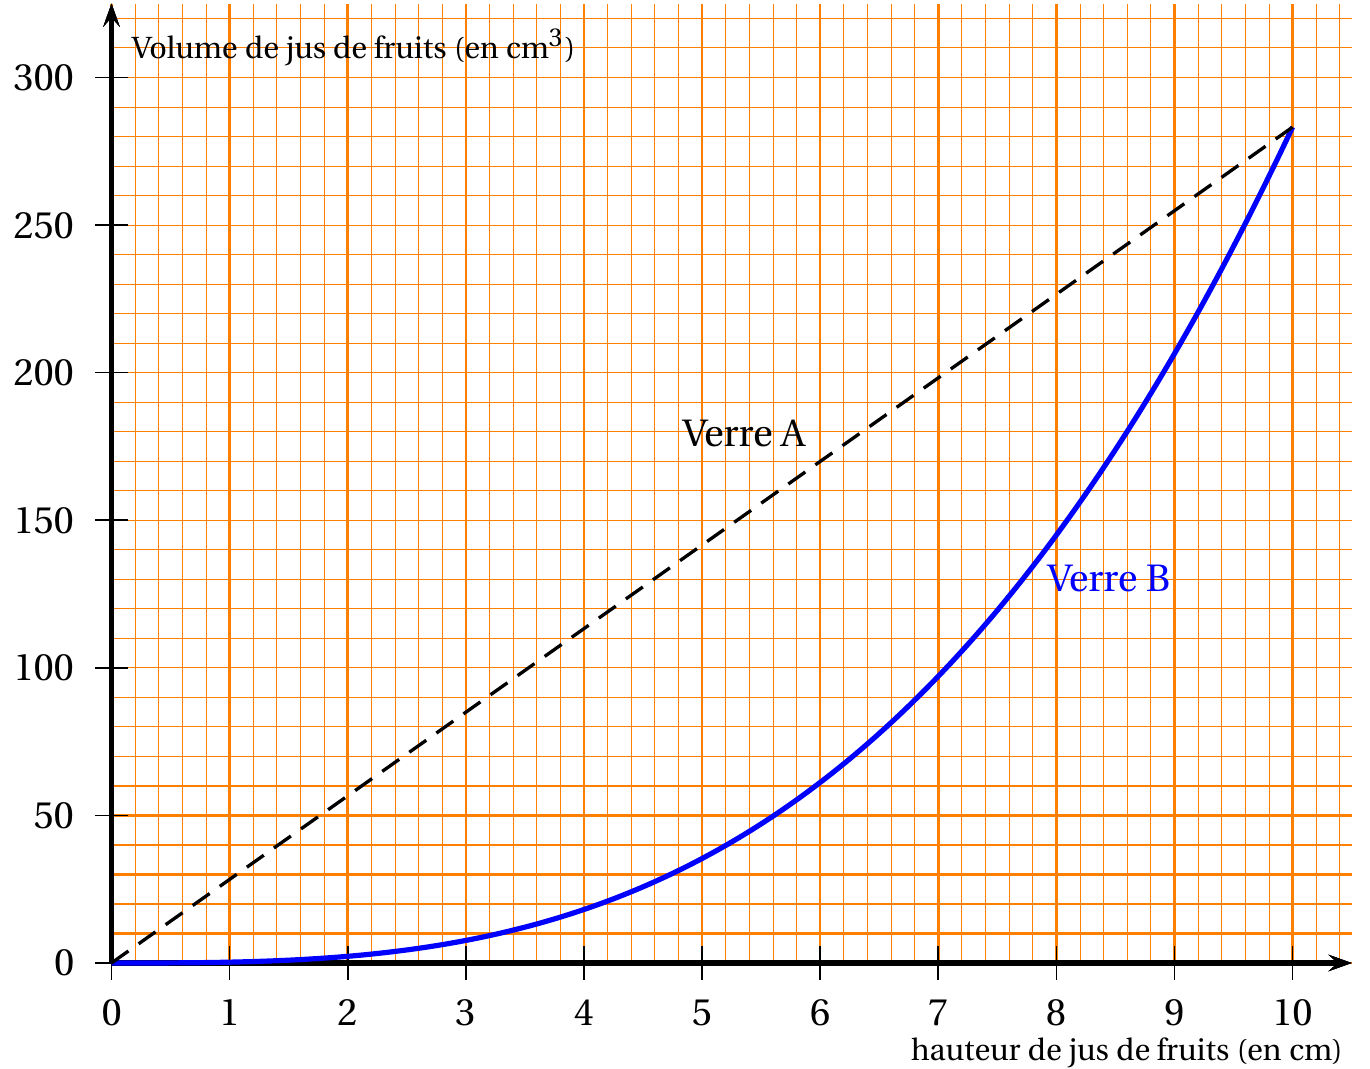
\includegraphics[scale=3]{Exo3.png}










\newpage


	 \begin{center} {\Large \textbf{Contôle fonctions}}
	 


\subsection*{Exercice 1}	 
	 
On considère une fonction $g$ dont un tableau de valeurs est le suivant : \begin{figure}[H]
\center
$\begin{array}{|c|c|c|c|c|c|}
\hline
 x &  -3 & -1 & 4 & 6  &  2 \\
\hline
g(x)&  5 & -3  & -4 & 14 &   2  \\
\hline
\end{array}$
\end{figure}	 

\begin{enumerate}
\item Donnez une image de $-3$ par $f$. 
\item Donnez un antécédent de $-3$ par $f$. 
\item Donnez un nombre tel que $f(x)= x$.
\end{enumerate}

\subsection*{Exercice 2 (9 points) }	 
	 
On considère le programme de calcul suivant : 
\begin{itemize}
\item Prendre un nombre
\item Retirer 3
\item Multiplier par le nombre de départ 
\item Ajouter 2
\end{itemize}
\begin{enumerate}
\item (2 pts) On note $h(x)$ le résultat du programme lorsqu'on choisit le nombre $x$ au départ. Donnez une expression algébrique de $h(x)$.
\item (1 pt) Calculez l'image de $1$ par $h$. 
\item (1 pt) Calculez l'image de $\frac12$ par $h$.
\item (3 pts) Remplir le tableau suivant : 
	 
\begin{figure}[H]
\center
$\begin{array}{|c|c|c|c|c|c|}
\hline
 x &  3 & -5 & \frac12 &    &   \\
\hline
h(x)&   & & & 0 &  2   \\
\hline
\end{array}$
\end{figure}
\item (2 pts) Développez et réduire l'expression de $h(x)$. 
\end{enumerate} 
\newpage

\subsection*{Exercice 3 (8 points) }\end{center}


Pour servir ses jus de fruits, un restaurateur a le choix entre deux types de verres :  - un verre cylindrique A de hauteur $10$~cm et de rayon $3$~cm\\ -un verre conique B de hauteur $10$~cm et de rayon $5,2$~cm.


Le graphique situé en \textbf{ANNEXE} représente le volume de jus de fruits dans chacun des verres en fonction de la hauteur de jus de fruits qu'ils contiennent.


\begin{enumerate}
\item[1)] (3 pts) Répondre aux questions suivantes à l'aide du graphique :
	\begin{enumerate}
		\item Pour quel verre le volume et la hauteur de jus de fruits sont-ils proportionnels ? Justifier.
		\item Pour le verre A, quel est le volume de jus de fruits si la hauteur est de $5$~cm ?
		\item Quelle est la hauteur de jus de fruits si on en verse $50$~cm$^3$ dans le verre B ?
 	\end{enumerate}
\item[2)] (2 pts)  Montrer, par le calcul, que les deux verres ont le même volume total à $1$ cm$^3$ près.
\item[3)] (1,5 pt) Calculer la hauteur du jus de fruits servi dans le verre A pour que le volume de jus soit égal à $200$~cm$^3$. Donner une valeur approchée au centimètre près.
\item[4)] (1,5 pt)  Un restaurateur sert ses verres de telle sorte que la hauteur du jus de fruits dans le verre soit égale à $8$~cm.
	\begin{enumerate}
		\item Par lecture graphique, déterminer quel type de verre le restaurateur doit choisir pour servir le plus grand nombre possible de verres avec 1 L de jus de fruits.
		\item Par le calcul, déterminer le nombre maximum de verres A qu'il pourra servir avec 1 L de jus de fruits.
	\end{enumerate}
\end{enumerate}

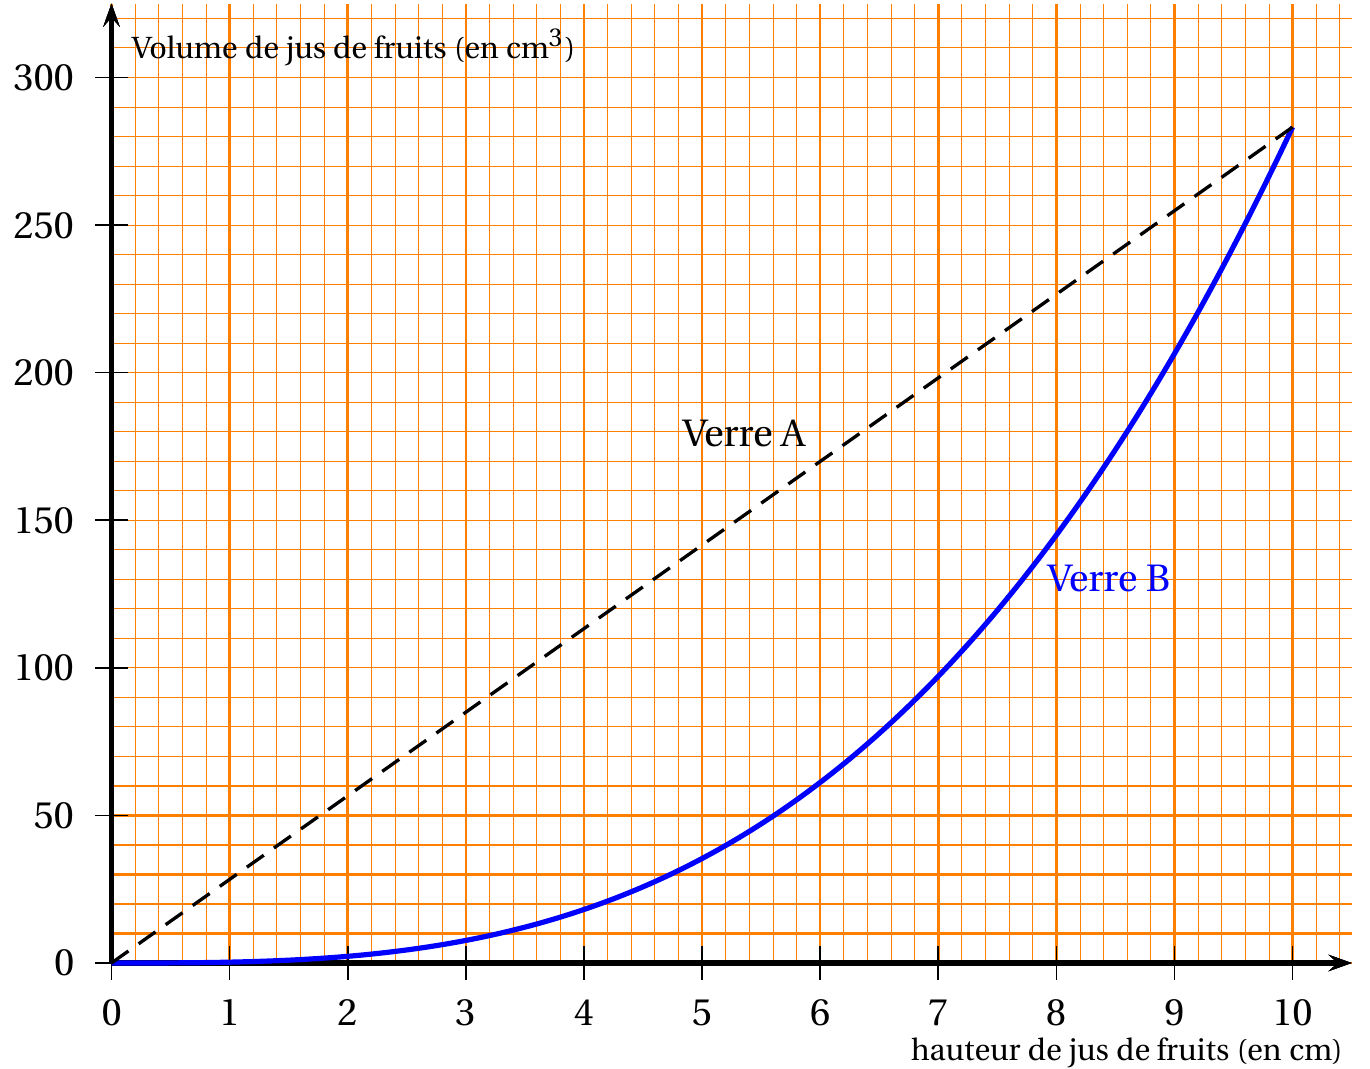
\includegraphics[scale=3]{Exo3.png}












    

 	\end{document}







